%package list
\documentclass{article}
\usepackage[top=3cm, bottom=3cm, outer=3cm, inner=3cm]{geometry}
\usepackage{multicol}
\usepackage{graphicx}
\usepackage{url}
%\usepackage{cite}
\usepackage{hyperref}
\usepackage{array}
%\usepackage{multicol}
\newcolumntype{x}[1]{>{\centering\arraybackslash\hspace{0pt}}p{#1}}
\usepackage{natbib}
\usepackage{pdfpages}
\usepackage{multirow}
\usepackage[normalem]{ulem}
\useunder{\uline}{\ul}{}
\usepackage{svg}
\usepackage{xcolor}
\usepackage{listings}
\lstdefinestyle{ascii-tree}{
    literate={├}{|}1 {─}{--}1 {└}{+}1 
  }
\lstset{basicstyle=\ttfamily,
  showstringspaces=false,
  commentstyle=\color{red},
  keywordstyle=\color{blue}
}
%\usepackage{booktabs}
\usepackage{caption}
\usepackage{subcaption}
\usepackage{float}
\usepackage{array}

\newcolumntype{M}[1]{>{\centering\arraybackslash}m{#1}}
\newcolumntype{N}{@{}m{0pt}@{}}


%%%%%%%%%%%%%%%%%%%%%%%%%%%%%%%%%%%%%%%%%%%%%%%%%%%%%%%%%%%%%%%%%%%%%%%%%%%%
%%%%%%%%%%%%%%%%%%%%%%%%%%%%%%%%%%%%%%%%%%%%%%%%%%%%%%%%%%%%%%%%%%%%%%%%%%%%
\newcommand{\itemEmail}{Diego Nina Suyo}
\newcommand{\itemStudent}{Javier Coronado Peña}
\newcommand{\itemCourse}{Estructura de Datos y Algoritmos}
\newcommand{\itemCourseCode}{20231001}
\newcommand{\itemSemester}{III}
\newcommand{\itemUniversity}{Universidad Nacional de San Agustín de Arequipa}
\newcommand{\itemFaculty}{Facultad de Ingeniería de Producción y Servicios}
\newcommand{\itemDepartment}{Departamento Académico de Ingeniería de Sistemas e Informática}
\newcommand{\itemSchool}{Escuela Profesional de Ingeniería de Sistemas}
\newcommand{\itemAcademic}{2023 - A}
\newcommand{\itemInput}{Del 16 Junio 2023}
\newcommand{\itemOutput}{Al 17 Junio 2023}
\newcommand{\itemPracticeNumber}{03}
\newcommand{\itemTheme}{Heap}
%%%%%%%%%%%%%%%%%%%%%%%%%%%%%%%%%%%%%%%%%%%%%%%%%%%%%%%%%%%%%%%%%%%%%%%%%%%%
%%%%%%%%%%%%%%%%%%%%%%%%%%%%%%%%%%%%%%%%%%%%%%%%%%%%%%%%%%%%%%%%%%%%%%%%%%%%

\usepackage[english,spanish]{babel}
\usepackage[utf8]{inputenc}
\AtBeginDocument{\selectlanguage{spanish}}
\renewcommand{\figurename}{Figura}
\renewcommand{\refname}{Referencias}
\renewcommand{\tablename}{Tabla} %esto no funciona cuando se usa babel
\AtBeginDocument{%
	\renewcommand\tablename{Tabla}
}

\usepackage{fancyhdr}
\pagestyle{fancy}
\fancyhf{}
\setlength{\headheight}{30pt}
\renewcommand{\headrulewidth}{1pt}
\renewcommand{\footrulewidth}{1pt}
\fancyhead[L]{\raisebox{-0.2\height}{
\includegraphics[width=3cm]{img/logo_episunsa.png}}}
\fancyhead[C]{\fontsize{7}{7}\selectfont	\itemUniversity \\ \itemFaculty \\ \itemDepartment \\ \itemSchool \\ \textbf{\itemCourse}}
\fancyhead[R]{\raisebox{-0.2\height}{
\includegraphics[width=1.2cm]{img/logo_abet}}}
\fancyfoot[L]{}
\fancyfoot[C]{\itemCourse}
\fancyfoot[R]{Página \thepage}

% para el codigo fuente
\usepackage{listings}
\usepackage{color, colortbl}
\definecolor{dkgreen}{rgb}{0,0.6,0}
\definecolor{gray}{rgb}{0.5,0.5,0.5}
\definecolor{mauve}{rgb}{0.58,0,0.82}
\definecolor{codebackground}{rgb}{0.95, 0.95, 0.92}
\definecolor{tablebackground}{rgb}{0.8, 0, 0}

\lstset{frame=tb,
	language=bash,
	aboveskip=3mm,
	belowskip=3mm,
	showstringspaces=false,
	columns=flexible,
	basicstyle={\small\ttfamily},
	numbers=none,
	numberstyle=\tiny\color{gray},
	keywordstyle=\color{blue},
	commentstyle=\color{dkgreen},
	stringstyle=\color{mauve},
	breaklines=true,
	breakatwhitespace=true,
	tabsize=3,
	backgroundcolor= \color{codebackground},
}

\begin{document}
	
	\vspace*{10px}
	
	\begin{center}	
		\fontsize{17}{17} \textbf{ Informe de la practica \itemPracticeNumber}
	\end{center}
	\centerline{\textbf{\Large Tema: \itemTheme}}
	%\vspace*{0.5cm}	

	\begin{flushright}
		\begin{tabular}{|M{2.5cm}|N|}
			\hline 
			\rowcolor{tablebackground}
			\color{white} \textbf{Nota}  \\
			\hline 
			     \\[30pt]
			\hline 			
		\end{tabular}
	\end{flushright}	

	\begin{table}[H]
		\begin{tabular}{|x{4.7cm}|x{4.8cm}|x{4.8cm}|}
			\hline 
			\rowcolor{tablebackground}
			\color{white} \textbf{Estudiante} & \color{white}\textbf{Escuela}  & \color{white}\textbf{Asignatura}   \\
			\hline 
			{\itemStudent \par \itemEmail} & \itemSchool & {\itemCourse \par Semestre: \itemSemester \par Código: \itemCourseCode}     \\
			\hline 			
		\end{tabular}
	\end{table}		
	
	\begin{table}[H]
		\begin{tabular}{|x{4.7cm}|x{4.8cm}|x{4.8cm}|}
			\hline 
			\rowcolor{tablebackground}
			\color{white}\textbf{Practica} & \color{white}\textbf{Tema}  & \color{white}\textbf{Duración}   \\
			\hline 
			\itemPracticeNumber & \itemTheme & -----   \\
			\hline 
		\end{tabular}
	\end{table}
	
	\begin{table}[H]
		\begin{tabular}{|x{4.7cm}|x{4.8cm}|x{4.8cm}|}
			\hline 
			\rowcolor{tablebackground}
			\color{white}\textbf{Semestre académico} & \color{white}\textbf{Fecha de inicio}  & \color{white}\textbf{Fecha de entrega}   \\
			\hline 
			\itemAcademic & \itemInput &  \itemOutput  \\
			\hline 
		\end{tabular}
	\end{table}
	\section{Consideraciones para la entrega}
	\begin{itemize}
		\item Ademas, deben de subir al aula virtual el archivo con el codigo realizado.
		\item El trabajo sera desarrollado en parejas, durante las horas de practica en aula.
		\item Las soluciones de los ejercicios deberán ser subidos a un repositorio en Github, que deben compartirlo
con el profesor. Limite de plazo para cualquier actualización que se realice hasta las 12.00 del medio del
sábado 17/06/2023.
		\item Además, un integrante del grupo debe subir al aula virtual el archivo con el código realizado, y el enlace
del repositorio de trabajo. Limite de plazo hasta el término de la sesión del viernes 16 de junio de 2023.
	
	\end{itemize}
		
	\section{Tarea}
	\begin{itemize}		
		\item Construya una cola de prioridad que utilice un heap como estructura de datos. Para esto realice
lo siguiente:
		\item Implemente el TAD Heap genérico que este almacenado sobre un ArrayList con las operaciones
de inserción y eliminación. Este TAD debe de ser un heap maximo.
		\item Implemente la clase PriorityQueueHeap generica que utilice como estructura de datos el heap
desarrollado en el punto anterior. Esta clase debe tener las operaciones de una cola tales como:
		\item Enqueue (x, p) : inserta un elemento a la cola ‘x’ de prioridad ‘p’ a la cola. Como la
cola esta sobre un heap, este deberá ser insertado en el heap-max y reubicado de
acuerdo a su prioridad.
		\item Dequeue() : elimina el elemento de la mayor prioridad y lo devuelve. Nuevamente
como la cola está sobre un heap-max, el elemento que debe ser eliminado es la raíz,
por tanto, deberá sustituir este elemento por algún otro de modo que se cumpla las
propiedades del heap-max.
		\item Front() : solo devuelve el elemento de mayor priorioridad.
		\item Back(): sólo devuelve el elemento de menor prioridad.
	\end{itemize}
		
	
	
	\section{URL de Repositorio Github}
	\begin{itemize}
		\item URL del Repositorio GitHub para clonar o recuperar.
		\item \url{https://github.com/Shavicho/Practica_Heaps_grupoA.git}
		
	\end{itemize}
	
	\section{Ejercicio 3}
	
	\subsection{Creando la clase generica Elemento}
	\begin{itemize}	
		\item Definimos una clase generica llamada Elemento. La clase elemento implementa la interfaz Comparable lo que permite comparar las instancias de esta clase entre si.
		\item La clase Elemento tiene 2 private, prioridad un numero entero el cual sera la prioridad del elemento y el elemento el cual es un tipo generico T, su funcion es representar al elemento real.
	\end{itemize}	
	\lstinputlisting[language=Java, caption={Elemento.java},numbers=left,]{src/Elemento.java}
	\begin{itemize}
		\item La clase sobrescribe el metodo compareTo de la interfaz Comparable, Su funcion es comparar 2 objetos elementos en funcion de sus prioridades y devuelve el resultado de la comparacion.
	\end{itemize}
	\subsection{Creando la clase Heap}
	\begin{itemize}
		\item La clase Heap implementa la interfaz HeapInterface, que define las operaciones básicas de un montículo. La implementación utiliza un ArrayList llamado heap para almacenar los elementos del Heap. A continuacion los metodos utilizados en esta clase.
		\item insertar(T elemento): Este metodo recibe un elemento de tipo T y lo agrega al Heap. Luego, se llama al metodo flotar(int indice) para asegurarse de que el elemento llegue hasta su posicion correcta dentro del Heap.
		\item eliminarMaximo(): Este metodo elimina y devuelve el elemento máximo del Heap, que es el elemento en la posicion raíz (indice 0). Primero, verifica si el Heap está vacio y, si es asi, lanza una excepción. Luego, guarda el elemento máximo en una variable maximo y lo elimina  del ArrayList heap. Si el Heap no está vacío, coloca un nuevo elemento en la posición raiz y llama al metodo hundir(int indice) para asegurarse de que el elemento hunda hasta su posicion correcta dentro del monticulo. Finalmente, se devuelve el elemento máximo guardado en la variable maximo.
		\item minimo(): Este método devuelve el elemento minimo del Heap. Para hacer esto busca y devuelve el elemento minimo en el Heap. Si el montículo está vacío, se lanza una excepcion.
		\item flotar(int indice): Este metodo toma un indice como parametro y hace que el elemento en ese indice suba en el Heap hasta alcanzar la posicion correcta. El metodo compara el elemento con su padre y, si es mayor, los intercambia. Luego, actualiza el indice y continua comparando con el padre hasta que se alcance la posición correcta.
		\item hundir(int indice): Este metodo toma un indice como parametro y hace que el elemento baje el Heap hasta alcanzar la posición correcta. El metodo compara el elemento con sus hijos izquierdo y derecho y, si alguno de los hijos es mayor, intercambia el elemento con el hijo mayor. Luego, actualiza el índice y continua comparando con los hijos hasta que se alcance la posición correcta.
	\end{itemize}
\lstinputlisting[language=Java, caption={Heap.java},numbers=left,]{src/Heap.java}

	\subsection{Creando la clase PriorityQueueHeap}
	\begin{itemize}
		\item La clase PriorityQueueHeap es una implementación de una cola de prioridad utilizando un Heap genérico. Esta clase implementa la interfaz PriQueHeaInt.
		\item Cada elemento en el montículo es un objeto Elemento, que contiene el elemento real y su prioridad,
		\item Metodos utilizados en esta clase.
		\item enqueue(T elemento, int prioridad): Este método recibe un elemento de tipo T y su prioridad, y lo inserta en el montículo como un objeto Elemento. Utiliza el método insertar() del montículo para realizar la inserción.
		\item dequeue(): Este método elimina y devuelve el elemento con la máxima prioridad de la cola. Utiliza el método eliminarMaximo() del montículo para obtener el elemento máximo y luego llama al método getElemento() en el elemento para obtener el elemento real.
		\item front(): Este método devuelve el elemento con la máxima prioridad de la cola sin eliminarlo. Utiliza el método obtenerMaximo() del montículo para obtener el elemento máximo y luego llama al método getElemento() en el elemento para obtener el elemento real.
		\item back(): Este método devuelve el elemento con la mínima prioridad de la cola. Utiliza el método obtenerMinimo() del montículo para obtener el elemento mínimo y luego llama al método getElemento() en el elemento para obtener el elemento real.
	\end{itemize}
	\lstinputlisting[language=Java, caption={PriorityQueueHeap.java},numbers=left,]{src/PriorityQueueHeap.java}
	\subsection{Main}
	\begin{itemize}
		\item En el main se ejecuta el programa, ingresando datos;
	\end{itemize}
	\lstinputlisting[language=Java, caption={HeapMain.java},numbers=left,]{src/HeapMain.java}
	
	\begin{itemize}
		\item Ejecucion del programa, mostrando los metodos solicitados por el ejercicio.
	\end{itemize}
	\begin{figure}[H]
		\centering
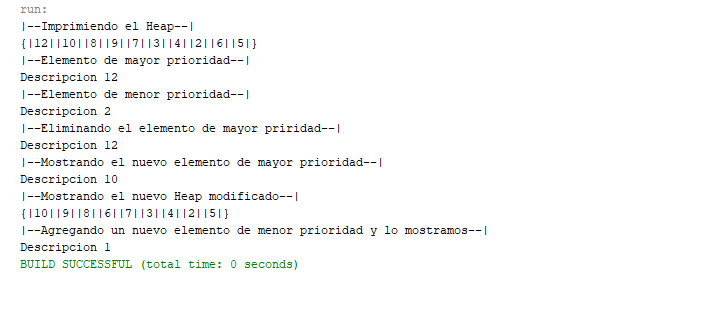
\includegraphics[width=0.8\textwidth,keepaspectratio]{img/ejecucion.png}
		%\includesvg{img/automata.svg}
		%\label{img:mot2}
		%\caption{Product backlog.}
	\end{figure}

	
	
%\clearpage
%\bibliographystyle{apalike}
%\bibliographystyle{IEEEtranN}
%\bibliography{bibliography}
			
\end{document}